\documentclass[language = czech]{webquiz}

\BreadCrumbs{Matematika https://www.math.muni.cz/\string~xvasicekm/
						| Matematicka analyza /https://www.math.muni.cz/\string~xvasicekm/analIndex.html/
						| title}

\InstitutionURL{https://www.math.muni.cz}

\title{Sudost a lichost funkce}

\usepackage[czech]{babel}
\usepackage{hyperref}
\usepackage[dvipdfmx]{graphicx}

\begin{document}
	
	\begin{discussion}[Sudost funkce]\label{d1} %Prometheus 
		\textbf{Funkce} $f$ se nazývá \textbf{sudá}, právě když zároveň platí:
		\begin{enumerate}
			\item Pro každé $x \in \text{D}_f$ je také $-x \in \text{D}_f$,
			\item Pro každé $x \in \text{D}_f$ je $f(-x)=f(x)$.
		\end{enumerate}
		Graf sudé funkce $y=x^2$\\
		\centering
		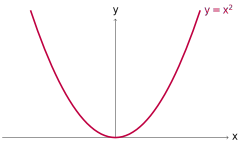
\includegraphics[scale=2]{x2.svg}
	\end{discussion}

	\begin{discussion}[Lichost funkce]\label{d2} %Prometheus 
			\textbf{Funkce} $f$ se nazývá \textbf{lichá}, právě když zároveň platí:
			
		\begin{enumerate}
			\item Pro každé $x \in \text{D}_f$ je také $-x \in \text{D}_f$,
			\item Pro každé $x \in \text{D}_f$ je $f(-x)=-f(x)$.
		\end{enumerate}
		
		Graf liché funkce $y=x^3$\\
		\centering
		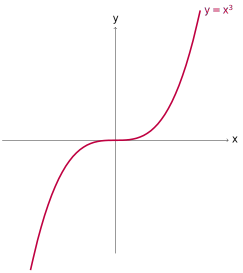
\includegraphics[scale=2]{x3.svg}
		
	\end{discussion}
	
	\begin{question} \label{o1} 
		Graf sudé funkce je?
		
		\begin{choice}[columns=2]
			\incorrect Osově souměrný podle osy $x$
				\feedback Zkus se podívat, jak vypadá graf \dref[sudé funkce]{d1}.
				
			\incorrect Středově souměrná se středem v bodě [0,0]
				\feedback Nepleť si \dref[sudou]{d1} a \dref[lichou]{d2} funkci.
				
			\incorrect Osově souměrná podle přímky $y=x$
				\feedback To platí o funkci inverzní, ale ne o sudé.
				
			\correct Osově souměrný podle osy $y$
				\feedback Skvělé! \qref[Další otázka]{o2}
				
		\end{choice}	
	\end{question}
	
	\begin{question} \label{o2}
		Mějme lichou funkci $f$. Funkční hodnota $f(2) = 8$, čemu se rovná $f(-2)$?
		
		\answer[integer]{-8}
		\whenRight Dobrá práce :) \qref[Další otázka]{o3}
		\whenWrong Zkus se podívat na \dref[definici liché funkce]{d2}.
	\end{question}
	
	\begin{question} \label{o3}
		Z nabídky grafů vyber grafy všech  funkcí, která jsou sudé.
			\begin{enumerate}
				\item 
\includegraphics[width = 1.9 cm]{sin.svg} 
				\item  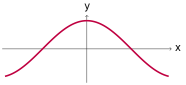
\includegraphics[width = 1.9 cm]{cos.svg}
				\item 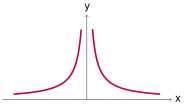
\includegraphics[width = 1.9 cm]{absfrac.svg}
				\item 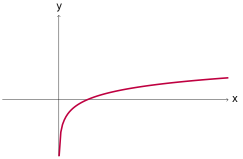
\includegraphics[width = 1.9 cm]{log.svg} 
			\end{enumerate}
		
		\begin{choice}[multiple, columns=4]
			\incorrect 1.  \feedback Škoda, zkus se kouknout na  \href{https://www.youtube.com/watch?v=6lFk55M3JXk}{video o sudoti a lichosti funkcí}.
			\correct 2. \feedback Dobrá práce, jen tak dál.
			\correct 3. \feedback Paráda :)
			\incorrect 4. \feedback Zopakuj si definice \dref[sudé]{d1} a \dref[liché]{d2} funkce.
		\end{choice}	
	\end{question}
	
	\begin{question} \label{o4}
		Která z nabízených funkcí je zároveň sudá i lichá?
		
		\begin{choice}
			
			\incorrect $f(x) = 2x$
				\feedback sudost: $f(x) = 2x, f(-x) = -2x \Rightarrow$ není sudá, protože $2x \neq -2x$\\ lichost: $f(x) = 2x, -f(-x) = -(-2x) = 2x \Rightarrow$ je lichá, protože $2x = 2x$.
			
			\correct $f(x) = 0$
				\feedback Správně!\\ Funkce je sudá, protože $f(x) = 0, f(-x) = 0$ a lichá, protože $f(x) = 0, -f(-x) = -(0) = 0$.
			
			\incorrect $f(x) = 4$
				\feedback sudost: $f(x) = 4, f(-x) = 4 \Rightarrow$ je sudá, protože $4 = 4$\\ lichost: $f(x) = 4, -f(-x) = -(4) = -4 \Rightarrow$ není lichá, protože $4 \neq -4$.
			
			\incorrect Taková funkce neexistuje
				\feedback Ale existuje. Zkus to znovu.
			
		\end{choice}	
	\end{question}
	
\end{document}























